%% Graph Coloring via Metaheuristic Optimization
%% OMfE 227-0707-00L · ETH Zürich · Spring 2026
%% Compile: pdflatex slides.tex  (run twice for references)

\documentclass[aspectratio=169,10pt]{beamer}

% ── Theme ────────────────────────────────────────────────────────────────────
\usetheme{Madrid}
\usecolortheme{default}

% ETH primary blue
\definecolor{ethblue}{RGB}{33,92,175}
\definecolor{ethgrey}{RGB}{111,111,111}
\definecolor{lightgrey}{RGB}{240,240,240}

\setbeamercolor{palette primary}{bg=ethblue,fg=white}
\setbeamercolor{palette secondary}{bg=ethblue!80,fg=white}
\setbeamercolor{palette tertiary}{bg=ethblue!60,fg=white}
\setbeamercolor{palette quaternary}{bg=ethblue,fg=white}
\setbeamercolor{structure}{fg=ethblue}
\setbeamercolor{frametitle}{bg=ethblue,fg=white}
\setbeamercolor{title}{bg=ethblue,fg=white}
\setbeamercolor{block title}{bg=ethblue,fg=white}
\setbeamercolor{block body}{bg=lightgrey}
\setbeamercolor{alerted text}{fg=ethblue}

\setbeamertemplate{navigation symbols}{}
\setbeamertemplate{footline}{%
  \leavevmode\hbox{%
    \begin{beamercolorbox}[wd=.33\paperwidth,ht=2.25ex,dp=1ex,center]{palette primary}%
      \usebeamerfont{author in head/foot}E.\ Aschmann \& M.\ Camenisch
    \end{beamercolorbox}%
    \begin{beamercolorbox}[wd=.34\paperwidth,ht=2.25ex,dp=1ex,center]{palette secondary}%
      \usebeamerfont{title in head/foot}Graph Coloring via Metaheuristics
    \end{beamercolorbox}%
    \begin{beamercolorbox}[wd=.33\paperwidth,ht=2.25ex,dp=1ex,right]{palette tertiary}%
      \usebeamerfont{date in head/foot}\insertframenumber{} / \inserttotalframenumber\hspace*{2ex}
    \end{beamercolorbox}%
  }%
}

% ── Packages ─────────────────────────────────────────────────────────────────
\usepackage{amsmath,amssymb}
\usepackage{booktabs}
\usepackage{graphicx}
\usepackage{tikz}
\usetikzlibrary{positioning,arrows.meta}
\usepackage{xcolor}
\usepackage{multirow}
\usepackage{array}
\usepackage{pgfplots}
\pgfplotsset{compat=1.18}
\usepackage{url}

% Algorithm colour palette (matching matplotlib / plots.py ALGO_COLORS)
\definecolor{algacolor}{RGB}{31,119,180}     % GA   blue
\definecolor{algaecolor}{RGB}{255,127,14}    % GAE  orange
\definecolor{algacocolor}{RGB}{44,160,44}    % ACO  green
\definecolor{algacolorsa}{RGB}{214,39,40}    % SA   red
\definecolor{hybridgacolor}{RGB}{227,119,194}% Hybrid GA+SA  pink   (#e377c2)
\definecolor{hybridacocolor}{RGB}{23,190,207}% Hybrid ACO+SA cyan   (#17becf)
\definecolor{dsatcolor}{RGB}{148,103,189}    % DSATUR purple

% ── Macros ───────────────────────────────────────────────────────────────────
\newcommand{\G}{\mathcal{G}}
\newcommand{\V}{\mathcal{V}}
\newcommand{\E}{\mathcal{E}}
\newcommand{\col}{c}
\newcommand{\kmax}{k_{\max}}
\newcommand{\kused}{k_{\text{used}}}
\newcommand{\viol}{v_{\text{viol}}}
\newcommand{\gap}{\Delta k}
\newcommand{\fitF}{F}

\newcommand{\algbox}[2]{\textcolor{#1}{\textbf{#2}}}

% ─────────────────────────────────────────────────────────────────────────────
\title[Graph Coloring via Metaheuristics]%
      {Graph Coloring via\\Metaheuristic Optimization}
\subtitle{GA · GAE · SA · ACO · Hybrid GA+SA · Hybrid ACO+SA}
\author{Elena Aschmann \and Mina Camenisch}
\institute{Optimization Methods for Engineers, 227-0707-00L\\ETH Zürich}
\date{Spring 2026}

% ═══════════════════════════════════════════════════════════════════════════
\begin{document}

% ── Slide 1: Title ───────────────────────────────────────────────────────────
\begin{frame}
\titlepage
\end{frame}

% ── Slide 2: Problem Description ─────────────────────────────────────────────
\begin{frame}{Problem: Graph Coloring}

\begin{columns}[T]
\begin{column}{0.52\textwidth}
\textbf{Given} an undirected graph $G = (V, E)$\\[0.5em]
\textbf{Find} an assignment $\col: V \to \{1,\ldots,k\}$ such that
\[
  \forall\,(u,v)\in E: \quad \col(u) \neq \col(v)
\]
\textbf{Minimize} $k$ — the \emph{chromatic number} $\chi(G)$\\[1em]

\begin{block}{Why it's hard}
$\chi(G)$ is NP-hard to compute exactly. Brute force: $O(k^{|V|})$.
\end{block}

\vspace{0.5em}
\textbf{Applications:} register allocation, scheduling, frequency assignment, map colouring
\end{column}

\begin{column}{0.44\textwidth}
\centering
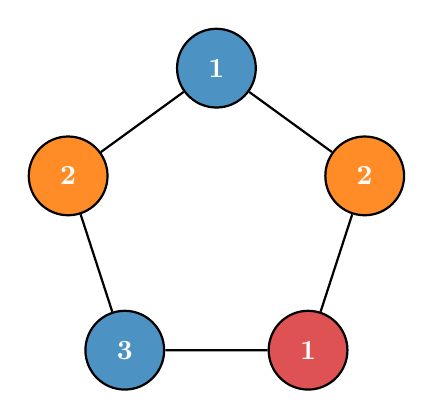
\begin{tikzpicture}[
  every node/.style={circle,draw,thick,minimum size=1cm,font=\bfseries},
  scale=1.1
]
  % A proper 3-coloring of C5
  \node[fill=algacolor!80,text=white]  (A) at (90:1.8)  {1};
  \node[fill=algaecolor!90,text=white] (B) at (18:1.8)  {2};
  \node[fill=algacolorsa!80,text=white](C) at (306:1.8) {1};
  \node[fill=algacolor!80,text=white]  (D) at (234:1.8) {3};
  \node[fill=algaecolor!90,text=white] (E) at (162:1.8) {2};
  \draw[thick] (A)--(B)--(C)--(D)--(E)--(A);
\end{tikzpicture}\\[0.3em]
{\small $C_5$: 3-coloring, $\chi(C_5)=3$}
\end{column}
\end{columns}

\end{frame}

% ── Slide 3: Mathematical Formulation ────────────────────────────────────────
\begin{frame}{Mathematical Formulation}

\begin{columns}[T]
\begin{column}{0.48\textwidth}
\begin{block}{Search Space}
\[
  \mathcal{S} = \{1,\ldots,\kmax\}^{|V|}, \quad |\mathcal{S}| = \kmax^{|V|}
\]
\end{block}

\vspace{0.5em}
\begin{block}{Fitness Function}
\[
  \fitF(\col) = \underbrace{\alpha\cdot\viol(\col)}_{\text{hard: feasibility}}
              + \underbrace{\beta\cdot\kused(\col)}_{\text{soft: minimise colours}}
\]
\[
  \alpha = 1000,\quad \beta = 1
\]
where $\viol(\col) = |\{(u,v)\in E : \col(u)=\col(v)\}|$
\end{block}

\vspace{0.5em}
$\alpha \gg \beta$ ensures any feasible solution beats any infeasible one.
\end{column}

\begin{column}{0.48\textwidth}
\begin{block}{Chromatic Gap (primary metric)}
\[
  \gap = \kused(\col^*) - \chi(G) \;\geq 0
\]
Lower is better. $\gap = 0$ is optimal.\\[0.5em]
In practice: $\chi(G)$ unknown for random graphs $\Rightarrow$ use DSATUR as reference.
\end{block}

\vspace{0.5em}
\begin{block}{Baselines}
\begin{tabular}{ll}
\textbf{BF} & Exact; exhaustive; $O(\kmax^n)$\\
\textbf{DSATUR} & Greedy; fast; reference for $\gap$
\end{tabular}
\end{block}
\end{column}
\end{columns}

\end{frame}

% ── Slide 4: Algorithm Overview ──────────────────────────────────────────────
\begin{frame}{Algorithms at a Glance}

\centering
\renewcommand{\arraystretch}{1.3}
\footnotesize
\begin{tabular}{>{\bfseries}l c c c l}
\toprule
Algorithm & Search strategy & State space & Init & Key idea \\
\midrule
\algbox{algacolor}{GA}
  & Population & $\{1,\ldots,k\}^n$ & Random & Crossover + mutation \\
\algbox{algaecolor}{GAE}
  & Population & $\{1,\ldots,k\}^n$ & Random & GA + elitism \\
\algbox{algacolorsa}{SA}
  & Single solution & $\{1,\ldots,k\}^n$ & Random & Metropolis acceptance + restarts \\
\algbox{algacocolor}{ACO}
  & Colony & $\{1,\ldots,k\}^n$ & Pheromone & Constructive; pheromone learning \\
\algbox{hybridgacolor}{GA+SA}
  & Population + local & $\{1,\ldots,k\}^n$ & Random & GA search, SA refines elites \\
\algbox{hybridacocolor}{ACO+SA}
  & Colony + local & $\{1,\ldots,k\}^n$ & Pheromone & ACO construction, SA refines best \\
\midrule
\textcolor{dsatcolor}{DSATUR}
  & Greedy & — & — & Baseline; max saturation-degree first \\
BF & Exhaustive & — & — & Optimal; $n \leq 10$ only \\
\bottomrule
\end{tabular}

\vspace{1em}
\normalsize
All metaheuristics share the same fitness $\fitF$ and the same interface:\\
$\texttt{run}(G,\, k_{\max},\, \text{params},\, \text{seed}) \to \text{AlgoResult}$

\end{frame}

% ── Slide 5: GA and GAE ───────────────────────────────────────────────────────
\begin{frame}{\algbox{algacolor}{GA} and \algbox{algaecolor}{GAE}: Genetic Algorithms}

\begin{columns}[T]
\begin{column}{0.50\textwidth}
\textbf{Encoding:} chromosome $\col \in \{1,\ldots,\kmax\}^n$, gene $i$ = colour of vertex $i$\\[0.7em]

\begin{enumerate}
  \item \textbf{Initialise} $N_{\text{pop}}$ random individuals
  \item \textbf{Evaluate} $\fitF(\col)$ for each
  \item \textbf{Repeat} for $N_{\text{gen}}$ generations:
    \begin{itemize}
      \item Tournament selection (size $t$)
      \item Two-point crossover with prob $p_{\text{cx}}$
      \item Per-gene mutation (uniform-int) with prob $p_{\text{mut}} \cdot p_{\text{ind}}$
      \item \textcolor{algaecolor}{[GAE] Reinject top $n_{\text{elite}}$ individuals}
    \end{itemize}
  \item \textbf{Return} best individual
\end{enumerate}

\end{column}

\begin{column}{0.46\textwidth}
\begin{block}{Tuned parameters}
\renewcommand{\arraystretch}{1.1}
\begin{tabular}{lcc}
\toprule
Parameter & \algbox{algacolor}{GA} & \algbox{algaecolor}{GAE} \\
\midrule
$N_{\text{pop}}$ & 100 & 100 \\
$p_{\text{cx}}$  & 0.90 & 1.00 \\
$p_{\text{mut}}$ & 0.50 & 0.50 \\
$p_{\text{ind}}$ & 0.05 & 0.05 \\
$N_{\text{gen}}$ & 200  & 200  \\
$n_{\text{elite}}$ & — & 3 \\
$t$              & 5    & 5    \\
\bottomrule
\end{tabular}
\end{block}
\vspace{0.3em}
{\small Tuned via OFAT sweep on $n \in \{40,50,60\}$, $p=0.5$}
\end{column}
\end{columns}

\end{frame}

% ── Slide 6: SA ──────────────────────────────────────────────────────────────
\begin{frame}{\algbox{algacolorsa}{SA}: Simulated Annealing with Restarts}

\begin{columns}[T]
\begin{column}{0.50\textwidth}
\begin{enumerate}
  \item \textbf{Initialise} randomly; set $T \leftarrow T_0$
  \item \textbf{Repeat} for $N_{\max}$ moves:
    \begin{itemize}
      \item Propose: reassign one vertex $i$ to colour $c' \neq \col(i)$
      \item Compute $\Delta\fitF$ incrementally in $O(\deg(i))$
      \item Accept with probability
        \[P = \min\!\left(1,\, e^{-\Delta\fitF / T}\right)\]
      \item Cool: every $n_{\text{step}}$ moves, $T \leftarrow \gamma T$
      \item \alert{Restart} to best-so-far if no improvement for $n_{\text{stall}}$ accepted moves
    \end{itemize}
  \item \textbf{Return} global best
\end{enumerate}
\end{column}

\begin{column}{0.46\textwidth}
\begin{block}{Tuned parameters}
\renewcommand{\arraystretch}{1.1}
\begin{tabular}{lc}
\toprule
Parameter & Value \\
\midrule
$T_0$         & 100 \\
$\gamma$      & 0.999 \\
$n_{\text{step}}$ & $5n$ \\
$n_{\text{stall}}$& 100 \\
$N_{\max}$    & $200 \cdot n_{\text{step}}$ \\
\bottomrule
\end{tabular}
\end{block}

\vspace{0.5em}
\textbf{Key property:} incremental $\Delta\fitF$ update makes each move $O(\deg(i))$ rather than $O(|E|)$.
Enables large $N_{\max}$ within tight time budget.
\end{column}
\end{columns}

\end{frame}

% ── Slide 7: ACO ─────────────────────────────────────────────────────────────
\begin{frame}{\algbox{algacocolor}{ACO}: Ant Colony Optimisation}

\begin{columns}[T]
\begin{column}{0.50\textwidth}
\textbf{Pheromone matrix} $\tau \in \mathbb{R}^{|V| \times k_{\max}}$:
$\tau_{ic}$ = desirability of assigning colour $c$ to vertex $i$\\[0.5em]

\textbf{Heuristic} (conflict avoidance):
\[
  \eta_{ic} = \frac{1}{1 + |\{j \in N(i) : \col(j)=c\}|}
\]

\textbf{Each ant constructs} a full colouring:
\[
  P(i,c) \;\propto\; \tau_{ic}^{\,\alpha} \cdot \eta_{ic}^{\,\beta}
\]
visiting vertices in a \emph{randomly shuffled} order.\\[0.5em]

\textbf{Pheromone update} (best-ant only):
\[
  \tau \leftarrow (1-\rho)\,\tau + \frac{Q}{\fitF_{\text{best}}} \cdot \mathbf{1}[\text{best ant}]
\]
\end{column}

\begin{column}{0.46\textwidth}
\begin{block}{Tuned parameters}
\renewcommand{\arraystretch}{1.1}
\begin{tabular}{lc}
\toprule
Parameter & Value \\
\midrule
$N_{\text{ants}}$ & 200 \\
$\alpha$          & 2.0 \\
$\beta$           & 5.0 \\
$\rho$            & 0.1 \\
$Q$               & 1.0 \\
$\tau_{\min}$     & 0.01 \\
$N_{\text{iter}}$ & 300 \\
\bottomrule
\end{tabular}
\end{block}

\vspace{0.5em}
High $\beta$ prioritises the heuristic (greedy conflict avoidance); each ant uses an \textbf{independent} vertex permutation for solution diversity.
\end{column}
\end{columns}

\end{frame}

% ── Slide 8: Hybrids ─────────────────────────────────────────────────────────
\begin{frame}{\algbox{hybridgacolor}{Hybrid GA+SA} and \algbox{hybridacocolor}{Hybrid ACO+SA}}

\begin{columns}[T]
\begin{column}{0.48\textwidth}
\textbf{\algbox{hybridgacolor}{GA+SA}:} standard GA population search; each generation, the elite individual(s) undergo a short SA local-search refinement pass before re-entering the population.\\[0.7em]

\textbf{\algbox{hybridacocolor}{ACO+SA}:} standard ACO pheromone-guided construction; once ants finish, the best-so-far colouring is refined by an SA local search with periodic restarts.\\[0.7em]

Both combine a global population/colony search with a cheap local-move refinement stage, aiming to reach better solutions than GA/ACO alone by polishing promising regions instead of only exploring globally.
\end{column}

\begin{column}{0.48\textwidth}
\begin{block}{Tuned parameters: \algbox{hybridgacolor}{GA+SA}}
\footnotesize
\renewcommand{\arraystretch}{0.9}
\begin{tabular}{lc}
\toprule
Parameter & Value \\
\midrule
$N_{\text{pop}}$, $N_{\text{gen}}$ & 80, 120 \\
$p_{\text{cx}}$, $p_{\text{mut}}$, $p_{\text{ind}}$ & 0.6, 0.4, 0.1 \\
$n_{\text{elite}}$, $t$ & 1, 4 \\
SA refine fraction & 0.2 \\
SA $T_0$, $\gamma$ & 1, 0.9 \\
\bottomrule
\end{tabular}
\end{block}

\vspace{0.3em}
\begin{block}{Tuned parameters: \algbox{hybridacocolor}{ACO+SA}}
\footnotesize
\renewcommand{\arraystretch}{0.9}
\begin{tabular}{lc}
\toprule
Parameter & Value \\
\midrule
$N_{\text{ants}}$, $N_{\text{iter}}$ & 20, 100 \\
$\alpha$, $\beta$, $\rho$ & 1, 3, 0.2 \\
SA restarts & 5 \\
SA $T_0$, $\gamma$ & 10, 0.9 \\
\bottomrule
\end{tabular}
\end{block}
\end{column}
\end{columns}

\end{frame}

% ── Slide 9: Experimental Setup ──────────────────────────────────────────────
\begin{frame}{Experimental Setup}

\begin{columns}[T]
\begin{column}{0.48\textwidth}
\begin{block}{Benchmark graphs}
\begin{itemize}
  \item Erdős–Rényi random graphs $G(n,p)$
  \item $n \in \{20, 30, 40, 50, 75, 100, 150, 200\}$
  \item $p \in \{0.3,\; 0.5,\; 0.7\}$
  \item $R = 20$ independent seeds per $(n, p)$
  \item Small-$n$ baseline: BF exact for $n \in \{8, 10\}$
\end{itemize}
\end{block}

\vspace{0.5em}
\begin{block}{Primary metric}
\[
  \text{gap}_{\text{DSATUR}} = \kused - k_{\text{DSATUR}}
\]
True $\chi(G)$ unknown $\Rightarrow$ DSATUR used as reference.\\
Negative gap = \emph{better} than DSATUR.
\end{block}
\end{column}

\begin{column}{0.48\textwidth}
\begin{block}{Infrastructure}
\begin{itemize}
  \item ETH piora cluster (SLURM)
  \item 1 job per $(n, p)$ combination (24 parallel jobs)
  \item 1 job per tuning combination (60 parallel jobs)
  \item Merging + analysis run locally
\end{itemize}
\end{block}

\vspace{0.5em}
\begin{block}{Tuning procedure}
\begin{itemize}
  \item OFAT sweep: one parameter varied at a time
  \item Fixed base: $n \in \{40,50,60\}$, $p=0.5$, $R=10$
  \item Best value selected by lowest mean $\gap$
\end{itemize}
\end{block}
\end{column}
\end{columns}

\end{frame}

% ── Slide 10: Results — Small n vs BF ─────────────────────────────────────────
\begin{frame}{Results: Optimality at Small $n$}

\begin{columns}[T]
\begin{column}{0.54\textwidth}
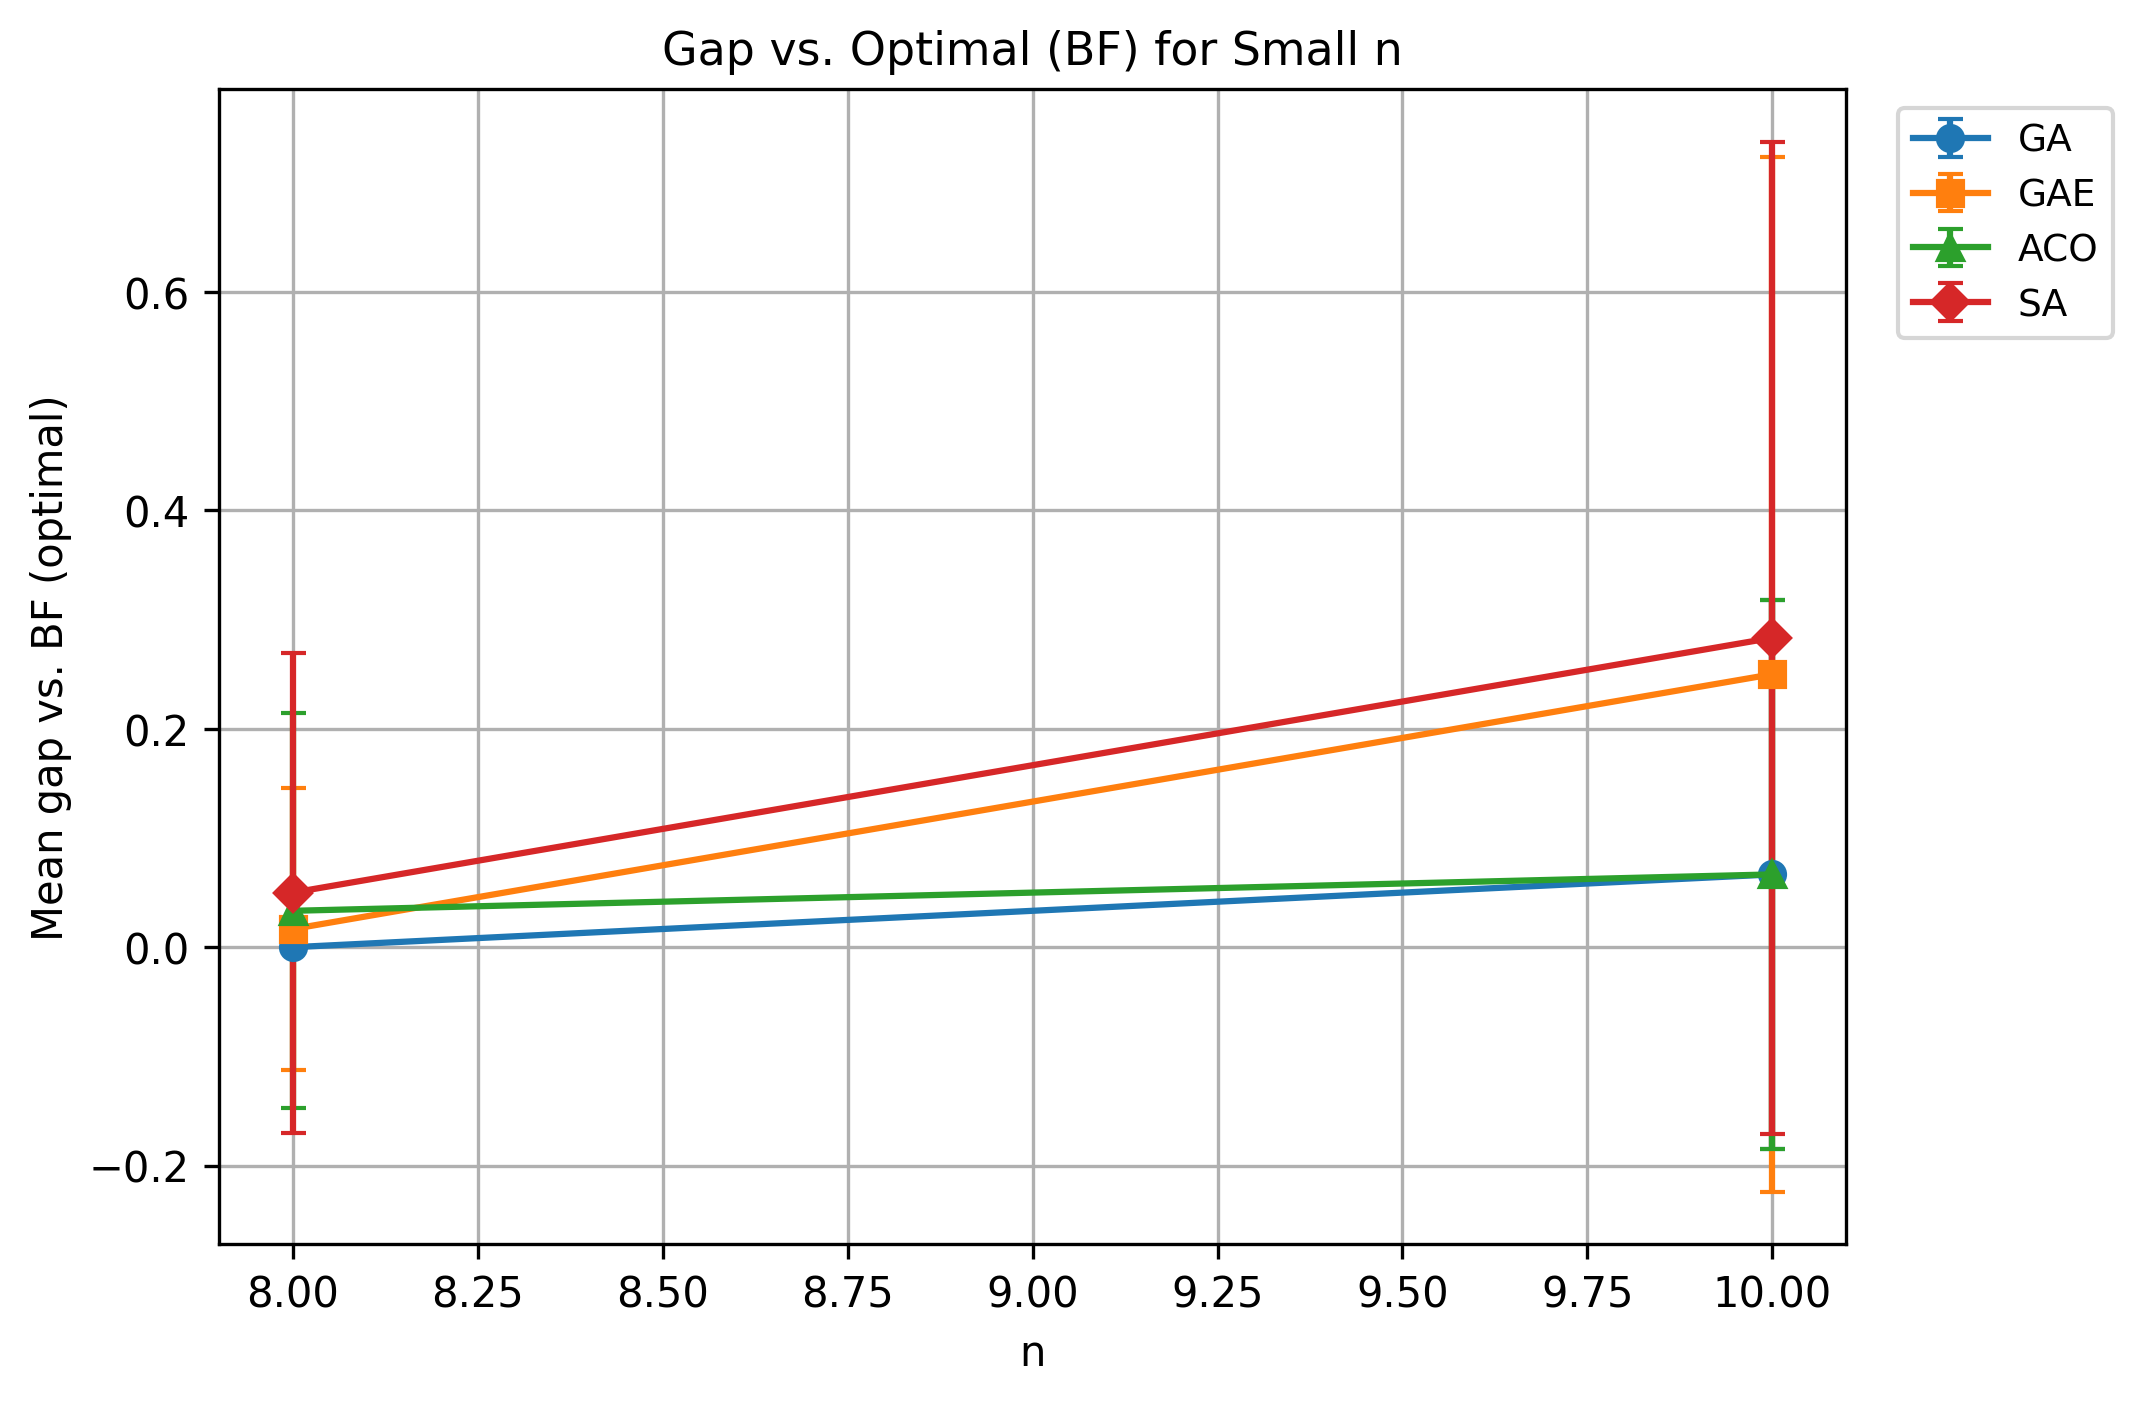
\includegraphics[width=\textwidth]{../results/figures/gap_vs_bf_small_n.png}
\end{column}

\begin{column}{0.43\textwidth}
\vspace{0.3em}
\textbf{Gap vs.\ exact optimum (BF)} for $n \in \{8, 10\}$\\[0.5em]

\begin{itemize}
  \item GA/GAE/SA/ACO all near-optimal; mean gap $\approx 0.1$ colours
  \item \textcolor{algacolor}{GA} closest to BF (0.03); \textcolor{algacolorsa}{SA} most variable (0.17, highest std)
  \item Negative gaps possible: occasionally beats DSATUR-seeded BF reference
  \item Hybrids not run at this scale (no BF comparison available)
\end{itemize}

\vspace{0.3em}
\begin{alertblock}{Takeaway}
GA, GAE, SA and ACO are all competitive with the exact solver when $n$ is small.
\end{alertblock}
\end{column}
\end{columns}

\end{frame}

% ── Slide 11: Results — Gap vs n ─────────────────────────────────────────────
\begin{frame}{Results: Scalability — Chromatic Gap vs.\ $n$}

\begin{columns}[T]
\begin{column}{0.54\textwidth}
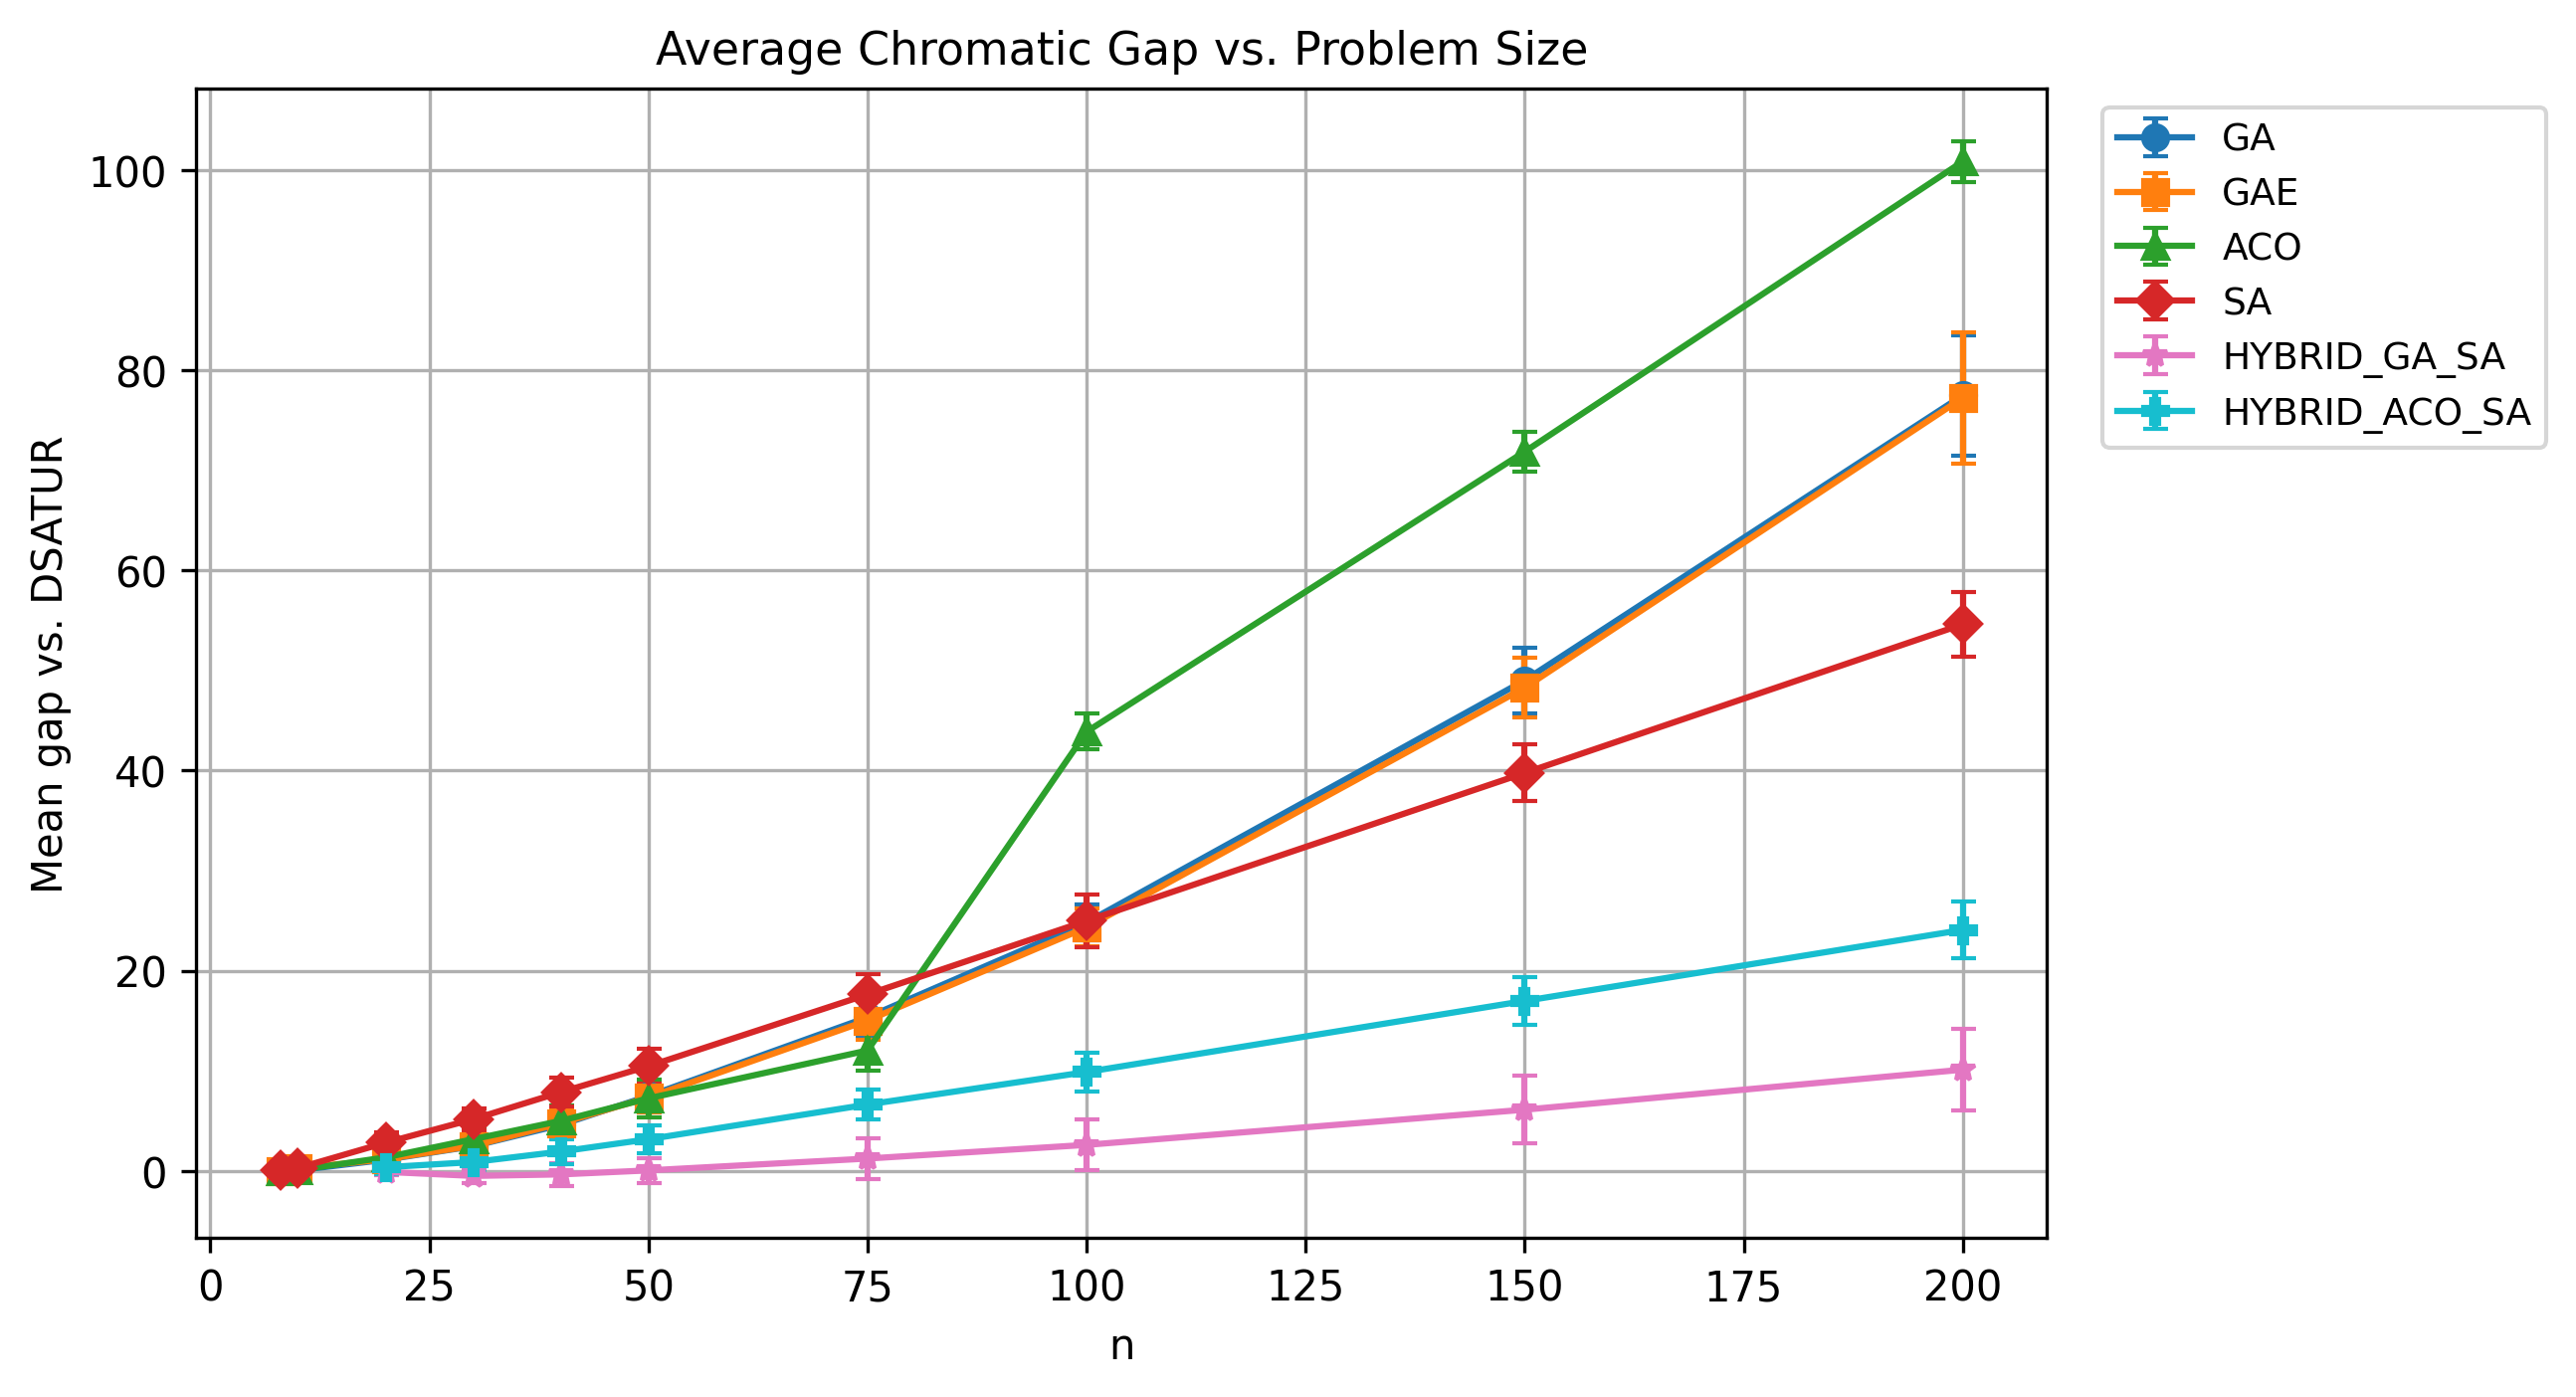
\includegraphics[width=\textwidth]{../results/figures/avg_gap_vs_n.png}
\end{column}

\begin{column}{0.43\textwidth}
\footnotesize
\vspace{0.2em}
Mean gap $\pm$ std over $p \in \{0.3,0.5,0.7\}$, $R=20$\\[0.3em]

\begin{itemize}
  \item \textcolor{hybridgacolor}{\textbf{Hybrid GA+SA}} best at every $n$, wide margin
  \item \textcolor{hybridacocolor}{Hybrid ACO+SA} distant 2nd, still far ahead of plain ACO
  \item Originals: \textcolor{algacolorsa}{SA} $<$ GA $\approx$ GAE $<$ \textcolor{algacocolor}{ACO}
  \item Gap grows roughly \emph{linearly} in $n$ for all six; hybrids' slopes are much shallower
\end{itemize}

\vspace{0.2em}
\begin{block}{At $n=200$}
\scriptsize
\renewcommand{\arraystretch}{0.8}
\begin{tabular}{lc}
\toprule
Algo & Mean gap \\
\midrule
\textcolor{hybridgacolor}{Hybrid GA+SA}  & \textbf{10.1} \\
\textcolor{hybridacocolor}{Hybrid ACO+SA}& 24.1 \\
\textcolor{algacolorsa}{SA} & 54.6 \\
\textcolor{algaecolor}{GAE} & 77.3 \\
\textcolor{algacolor}{GA}   & 77.5 \\
\textcolor{algacocolor}{ACO}& 100.9 \\
\bottomrule
\end{tabular}
\end{block}
\normalsize
\end{column}
\end{columns}

\end{frame}

% ── Slide 12: Results — Runtime and Convergence ───────────────────────────────
\begin{frame}{Results: Runtime and Convergence}

\begin{columns}[T]
\begin{column}{0.49\textwidth}
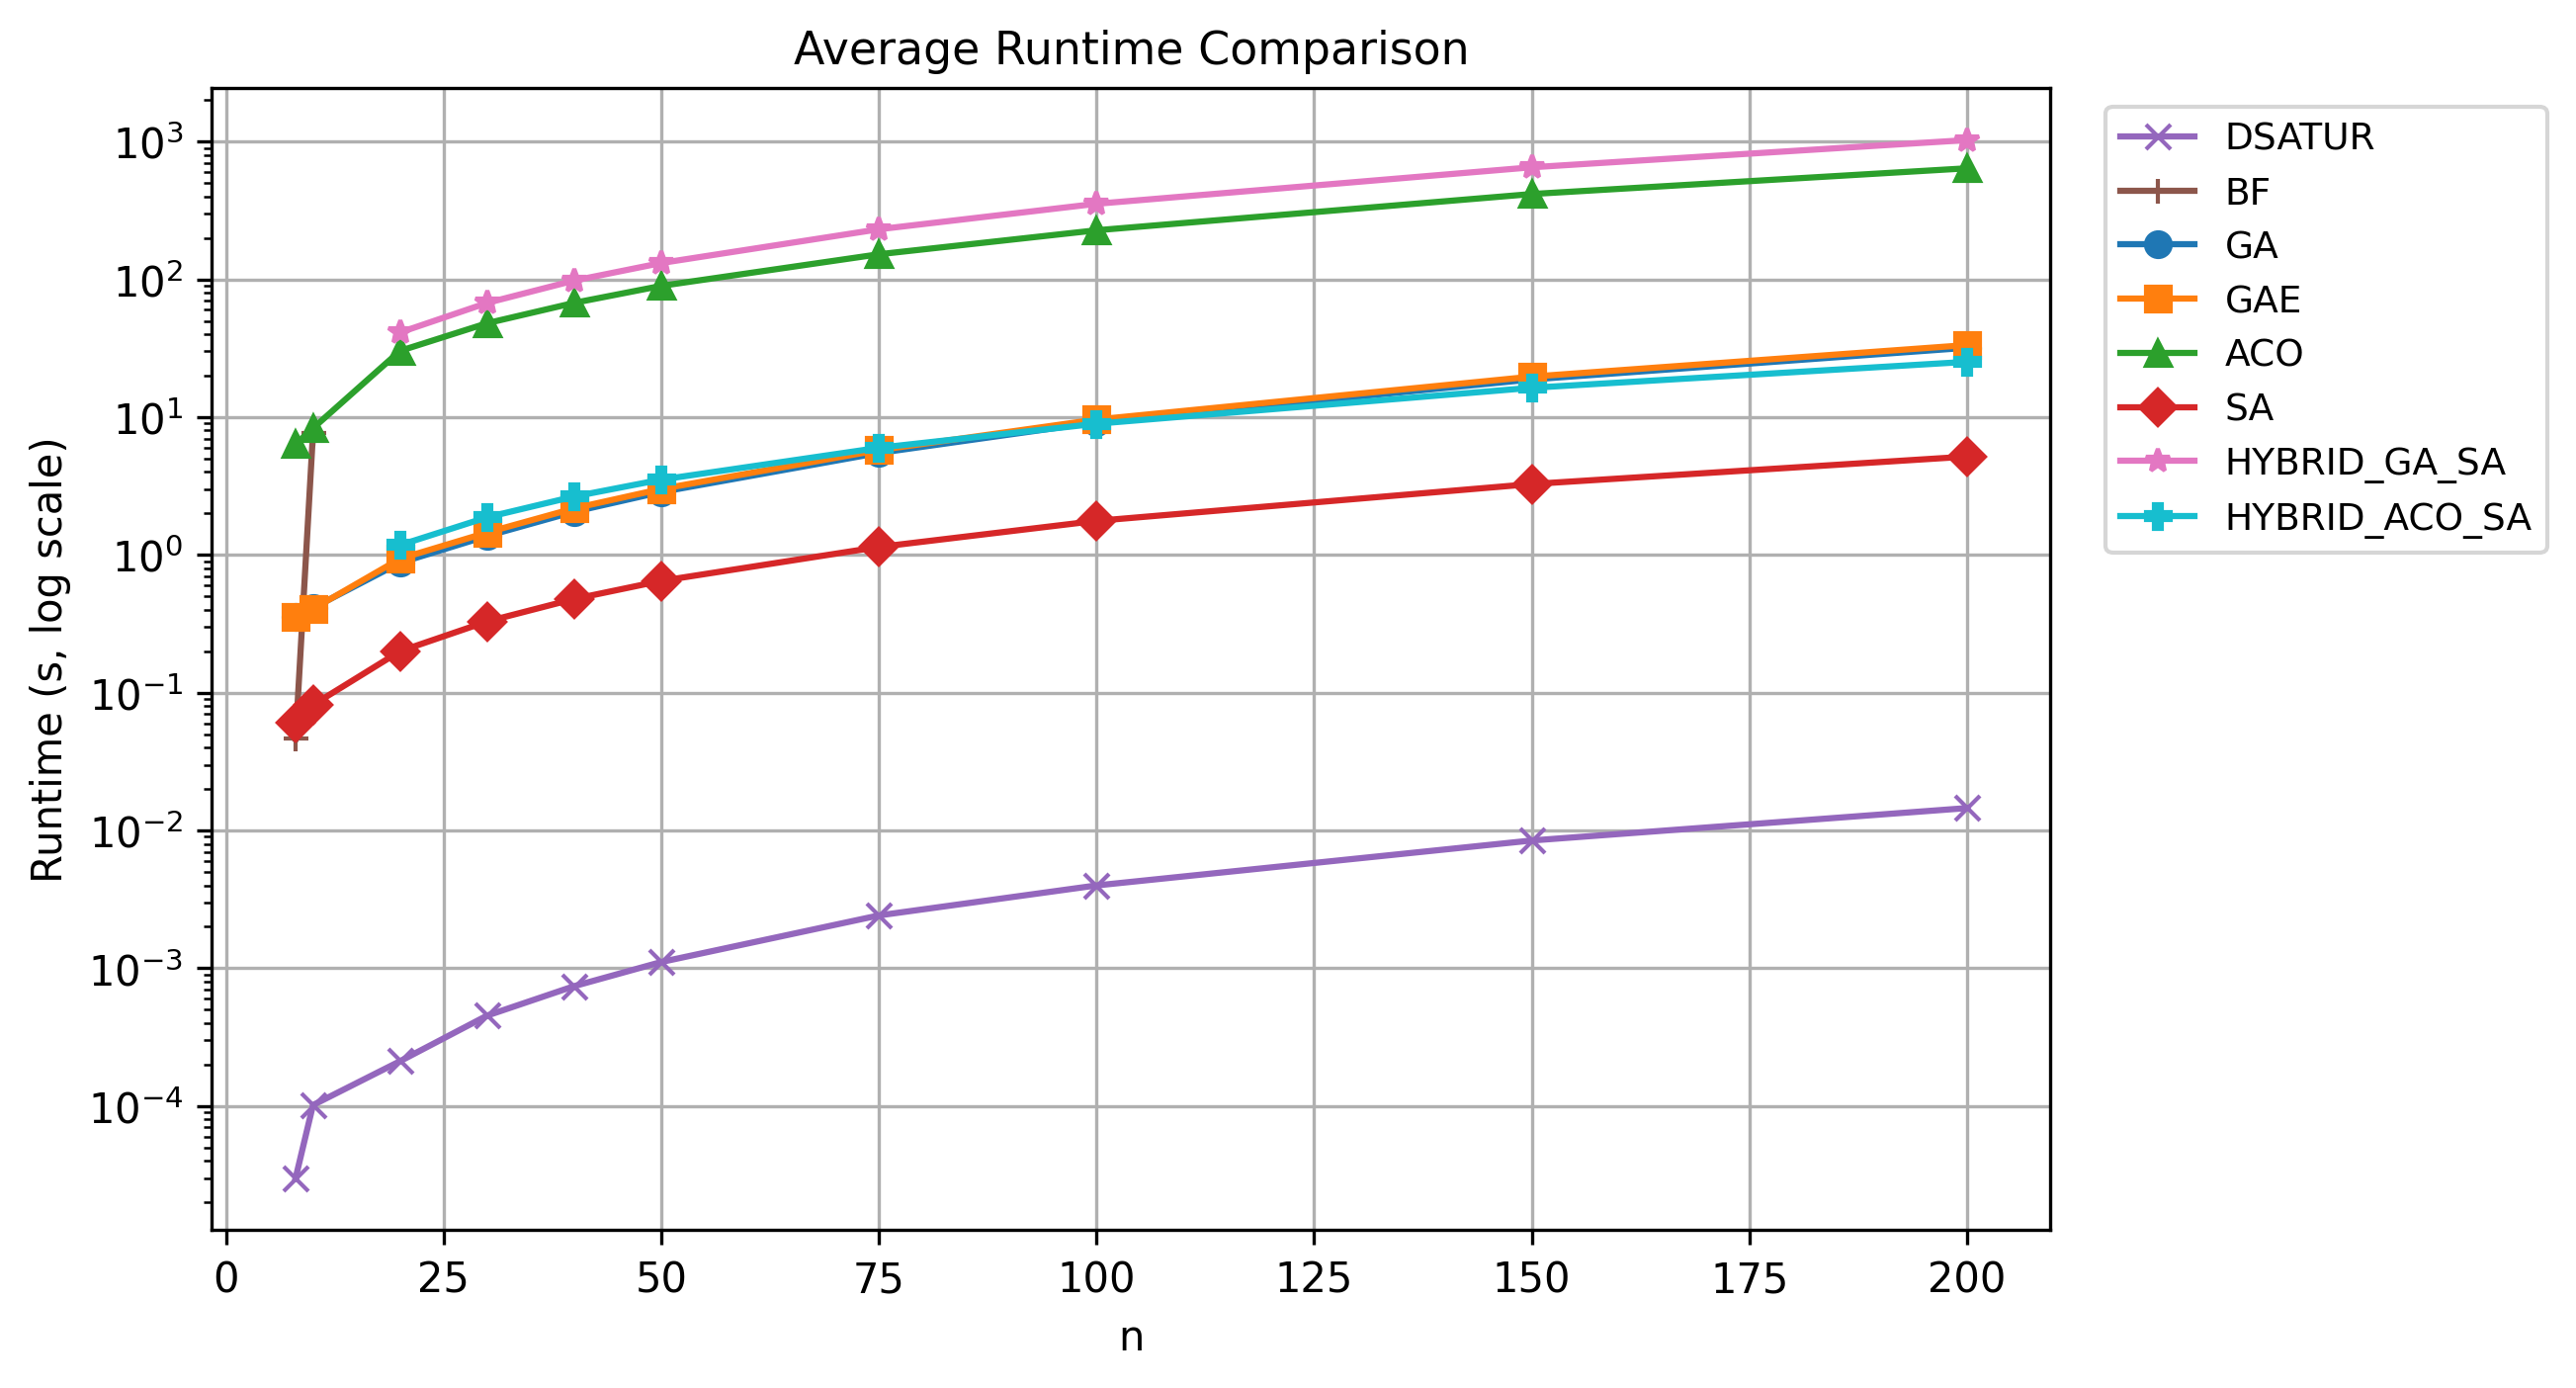
\includegraphics[width=\textwidth]{../results/figures/avg_runtime.png}\\[0.3em]
{\small Average wall-clock time, log scale}
\end{column}
\begin{column}{0.49\textwidth}
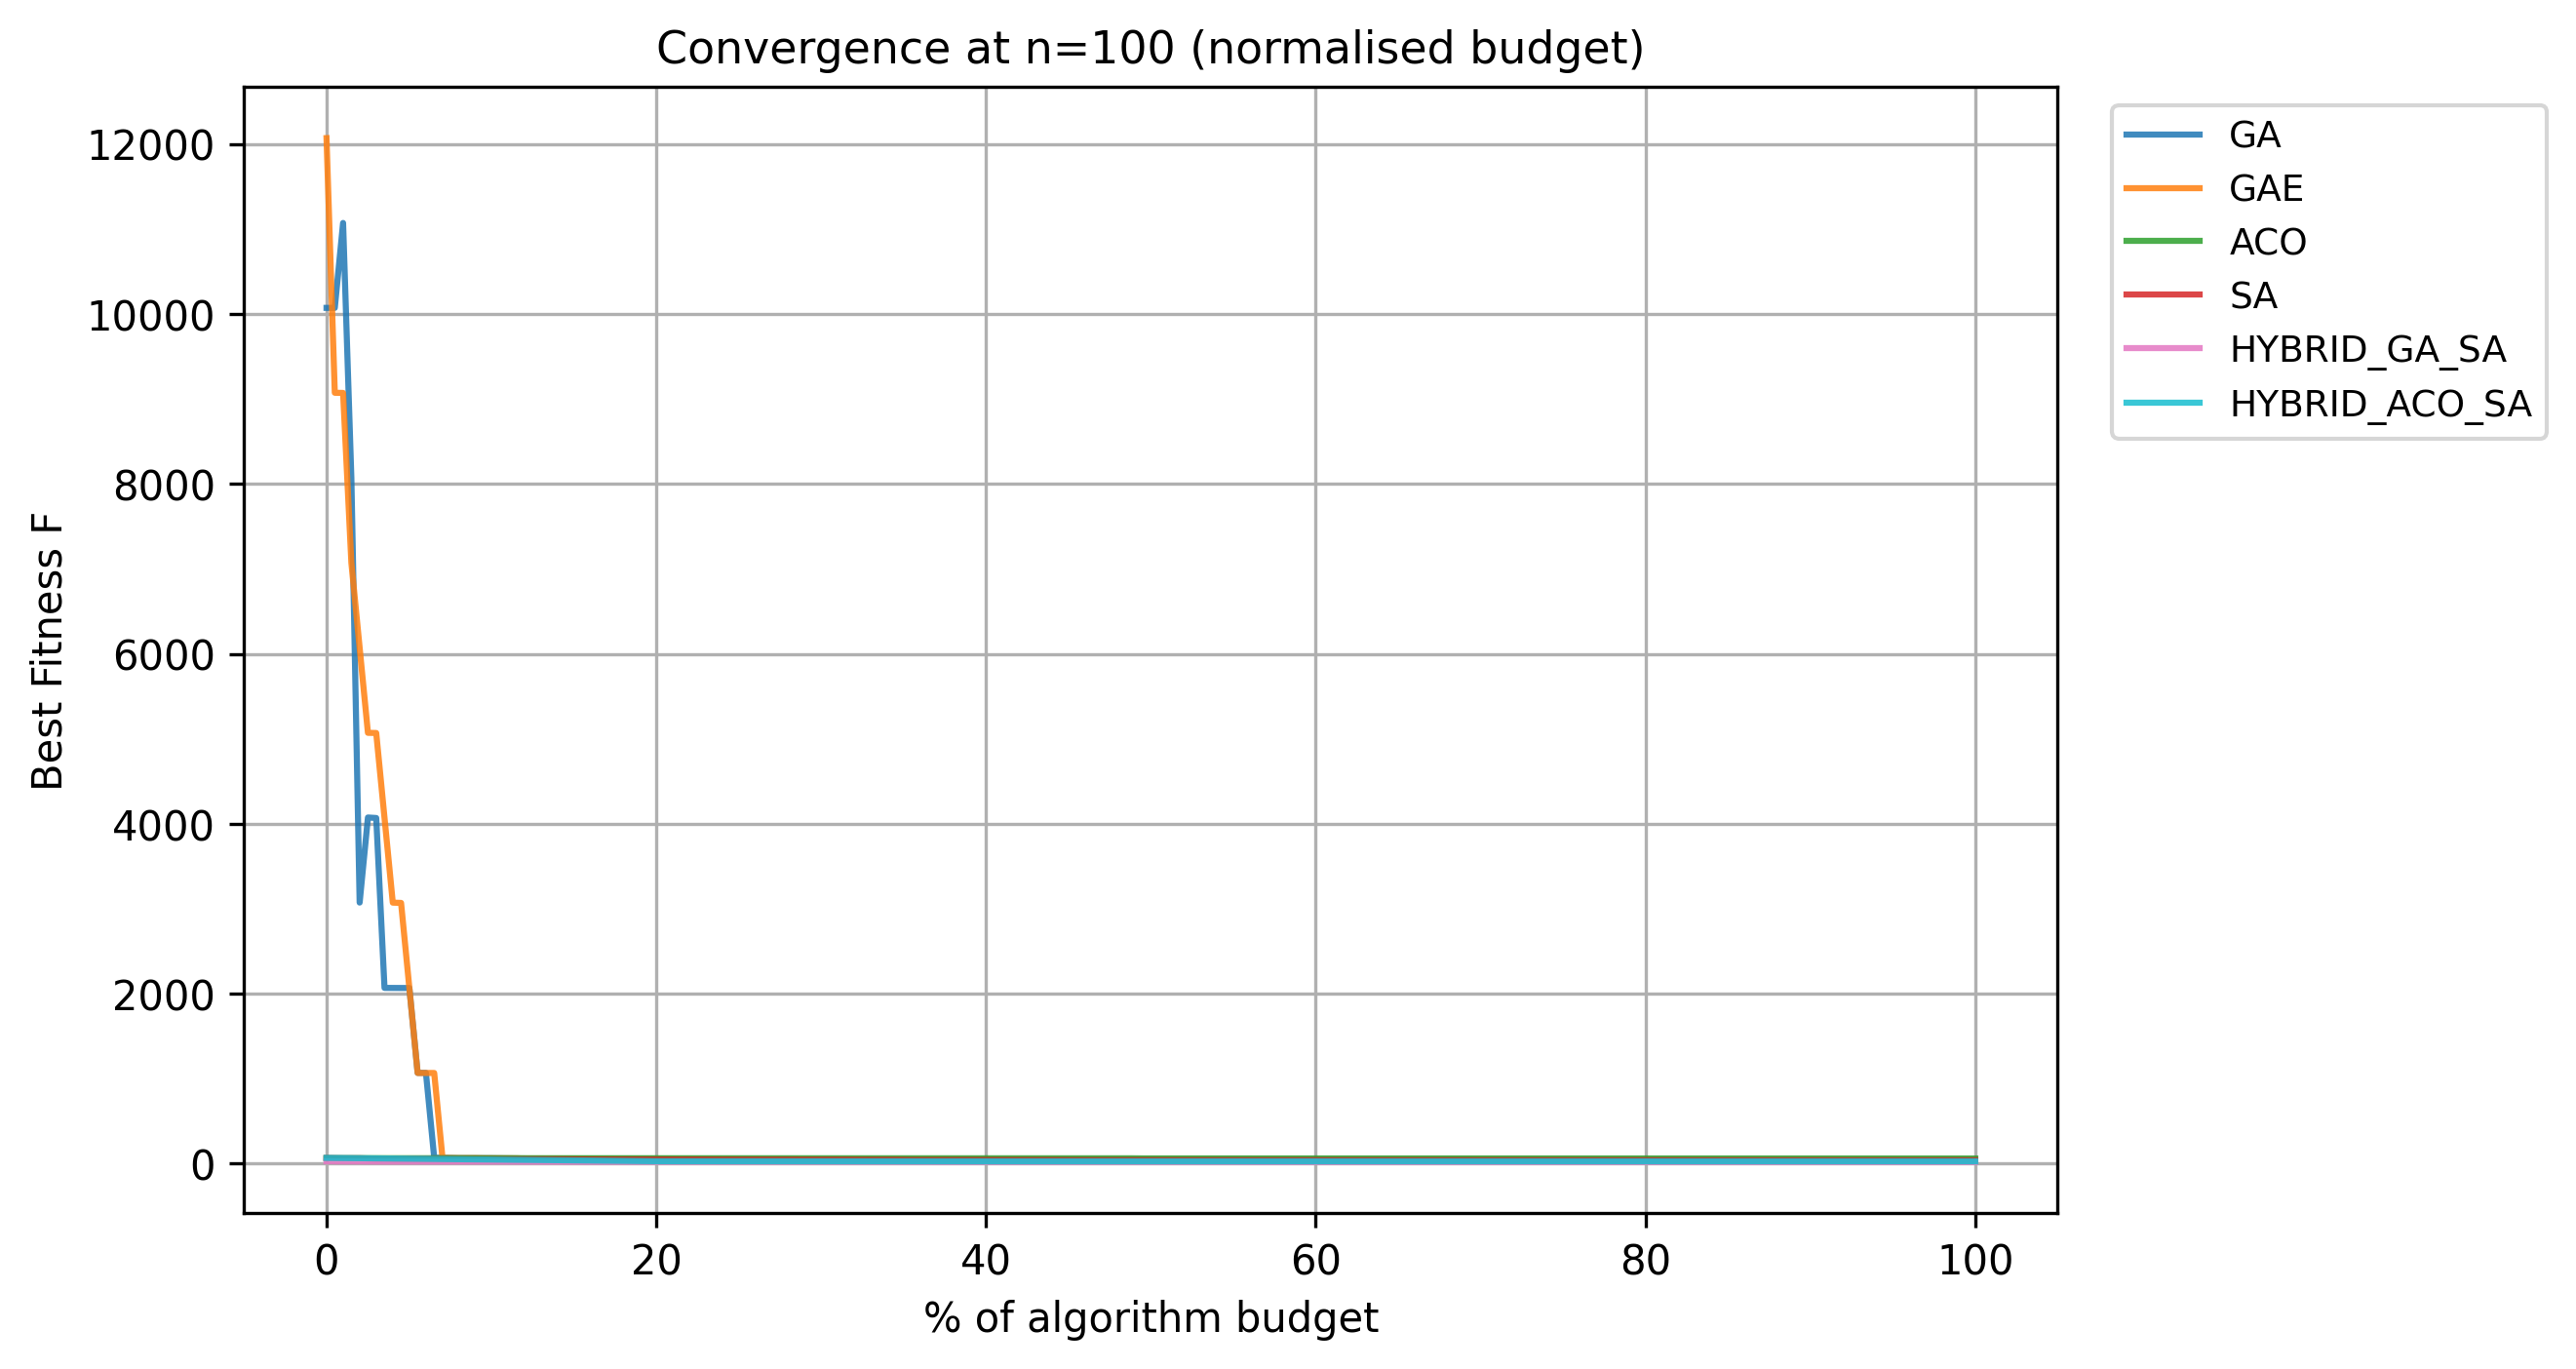
\includegraphics[width=\textwidth]{../results/figures/convergence_n100.png}\\[0.3em]
{\small Best fitness $\fitF$ vs.\ \% of budget ($G(100,\,0.5)$)}
\end{column}
\end{columns}

\vspace{0.2em}
\footnotesize
\begin{itemize}
  \item \textcolor{dsatcolor}{DSATUR} $10^3$–$10^5\times$ faster than any metaheuristic; \textcolor{algacolorsa}{SA} fastest metaheuristic ($\sim$\,5s at $n{=}200$)
  \item \textcolor{algacocolor}{ACO}, \textcolor{algacolorsa}{SA} and \textbf{both hybrids} start near-feasible; \textcolor{algacolor}{GA}/\textcolor{algaecolor}{GAE} start at $\fitF{\approx}11$–$12$k and need $\sim$\,8\,\% of budget to reach feasibility, then all plateau early
  \item \textcolor{hybridgacolor}{Hybrid GA+SA}: best quality overall but \emph{slowest} algorithm ($\sim$\,1026s at $n{=}200$) — its per-generation SA pass dominates runtime
  \item \textcolor{hybridacocolor}{Hybrid ACO+SA}: better trade-off — $\sim$\,4$\times$ ACO's quality at $\sim$\,25\,\% of ACO's runtime ($\sim$\,25s vs.\ $\sim$\,640s)
\end{itemize}
\normalsize

\end{frame}

% ── Slide 13: Results — Variance and Density ─────────────────────────────────
\begin{frame}{Results: Variance and Effect of Graph Density}

\begin{columns}[T]
\begin{column}{0.49\textwidth}
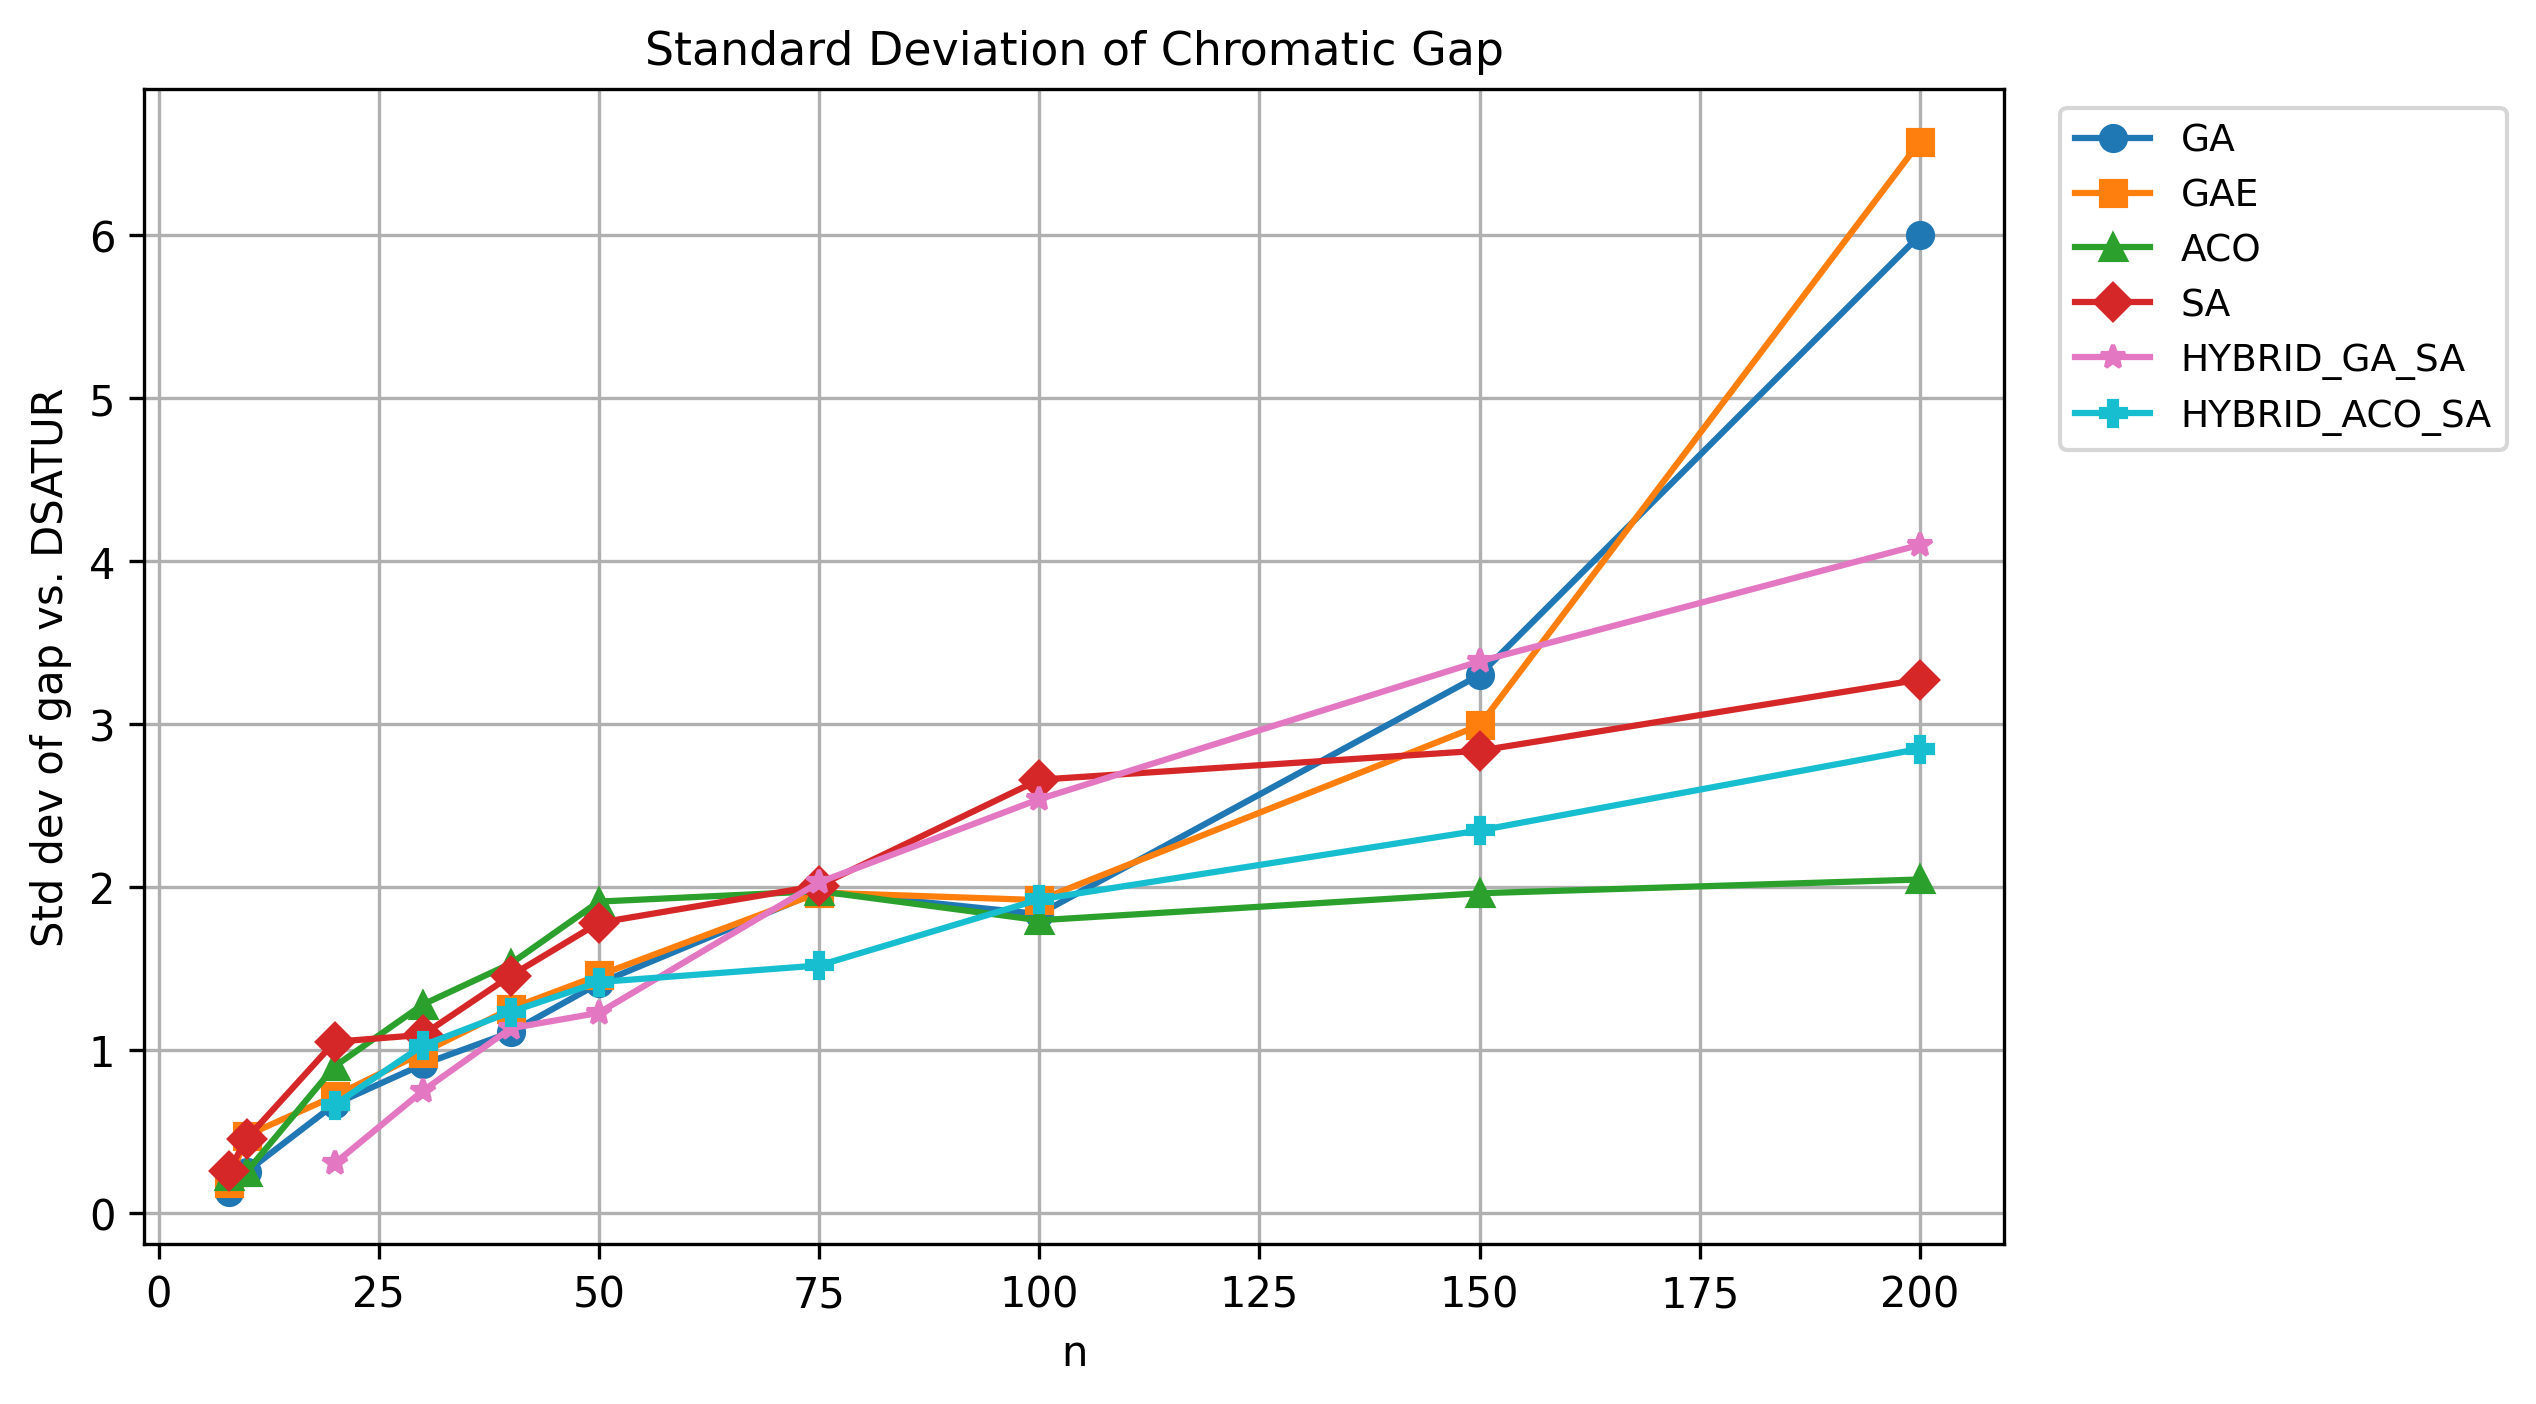
\includegraphics[width=\textwidth]{../results/figures/std_dev_gap.png}\\[0.3em]
{\small Std.\ dev.\ of gap vs.\ $n$}
\end{column}
\begin{column}{0.49\textwidth}
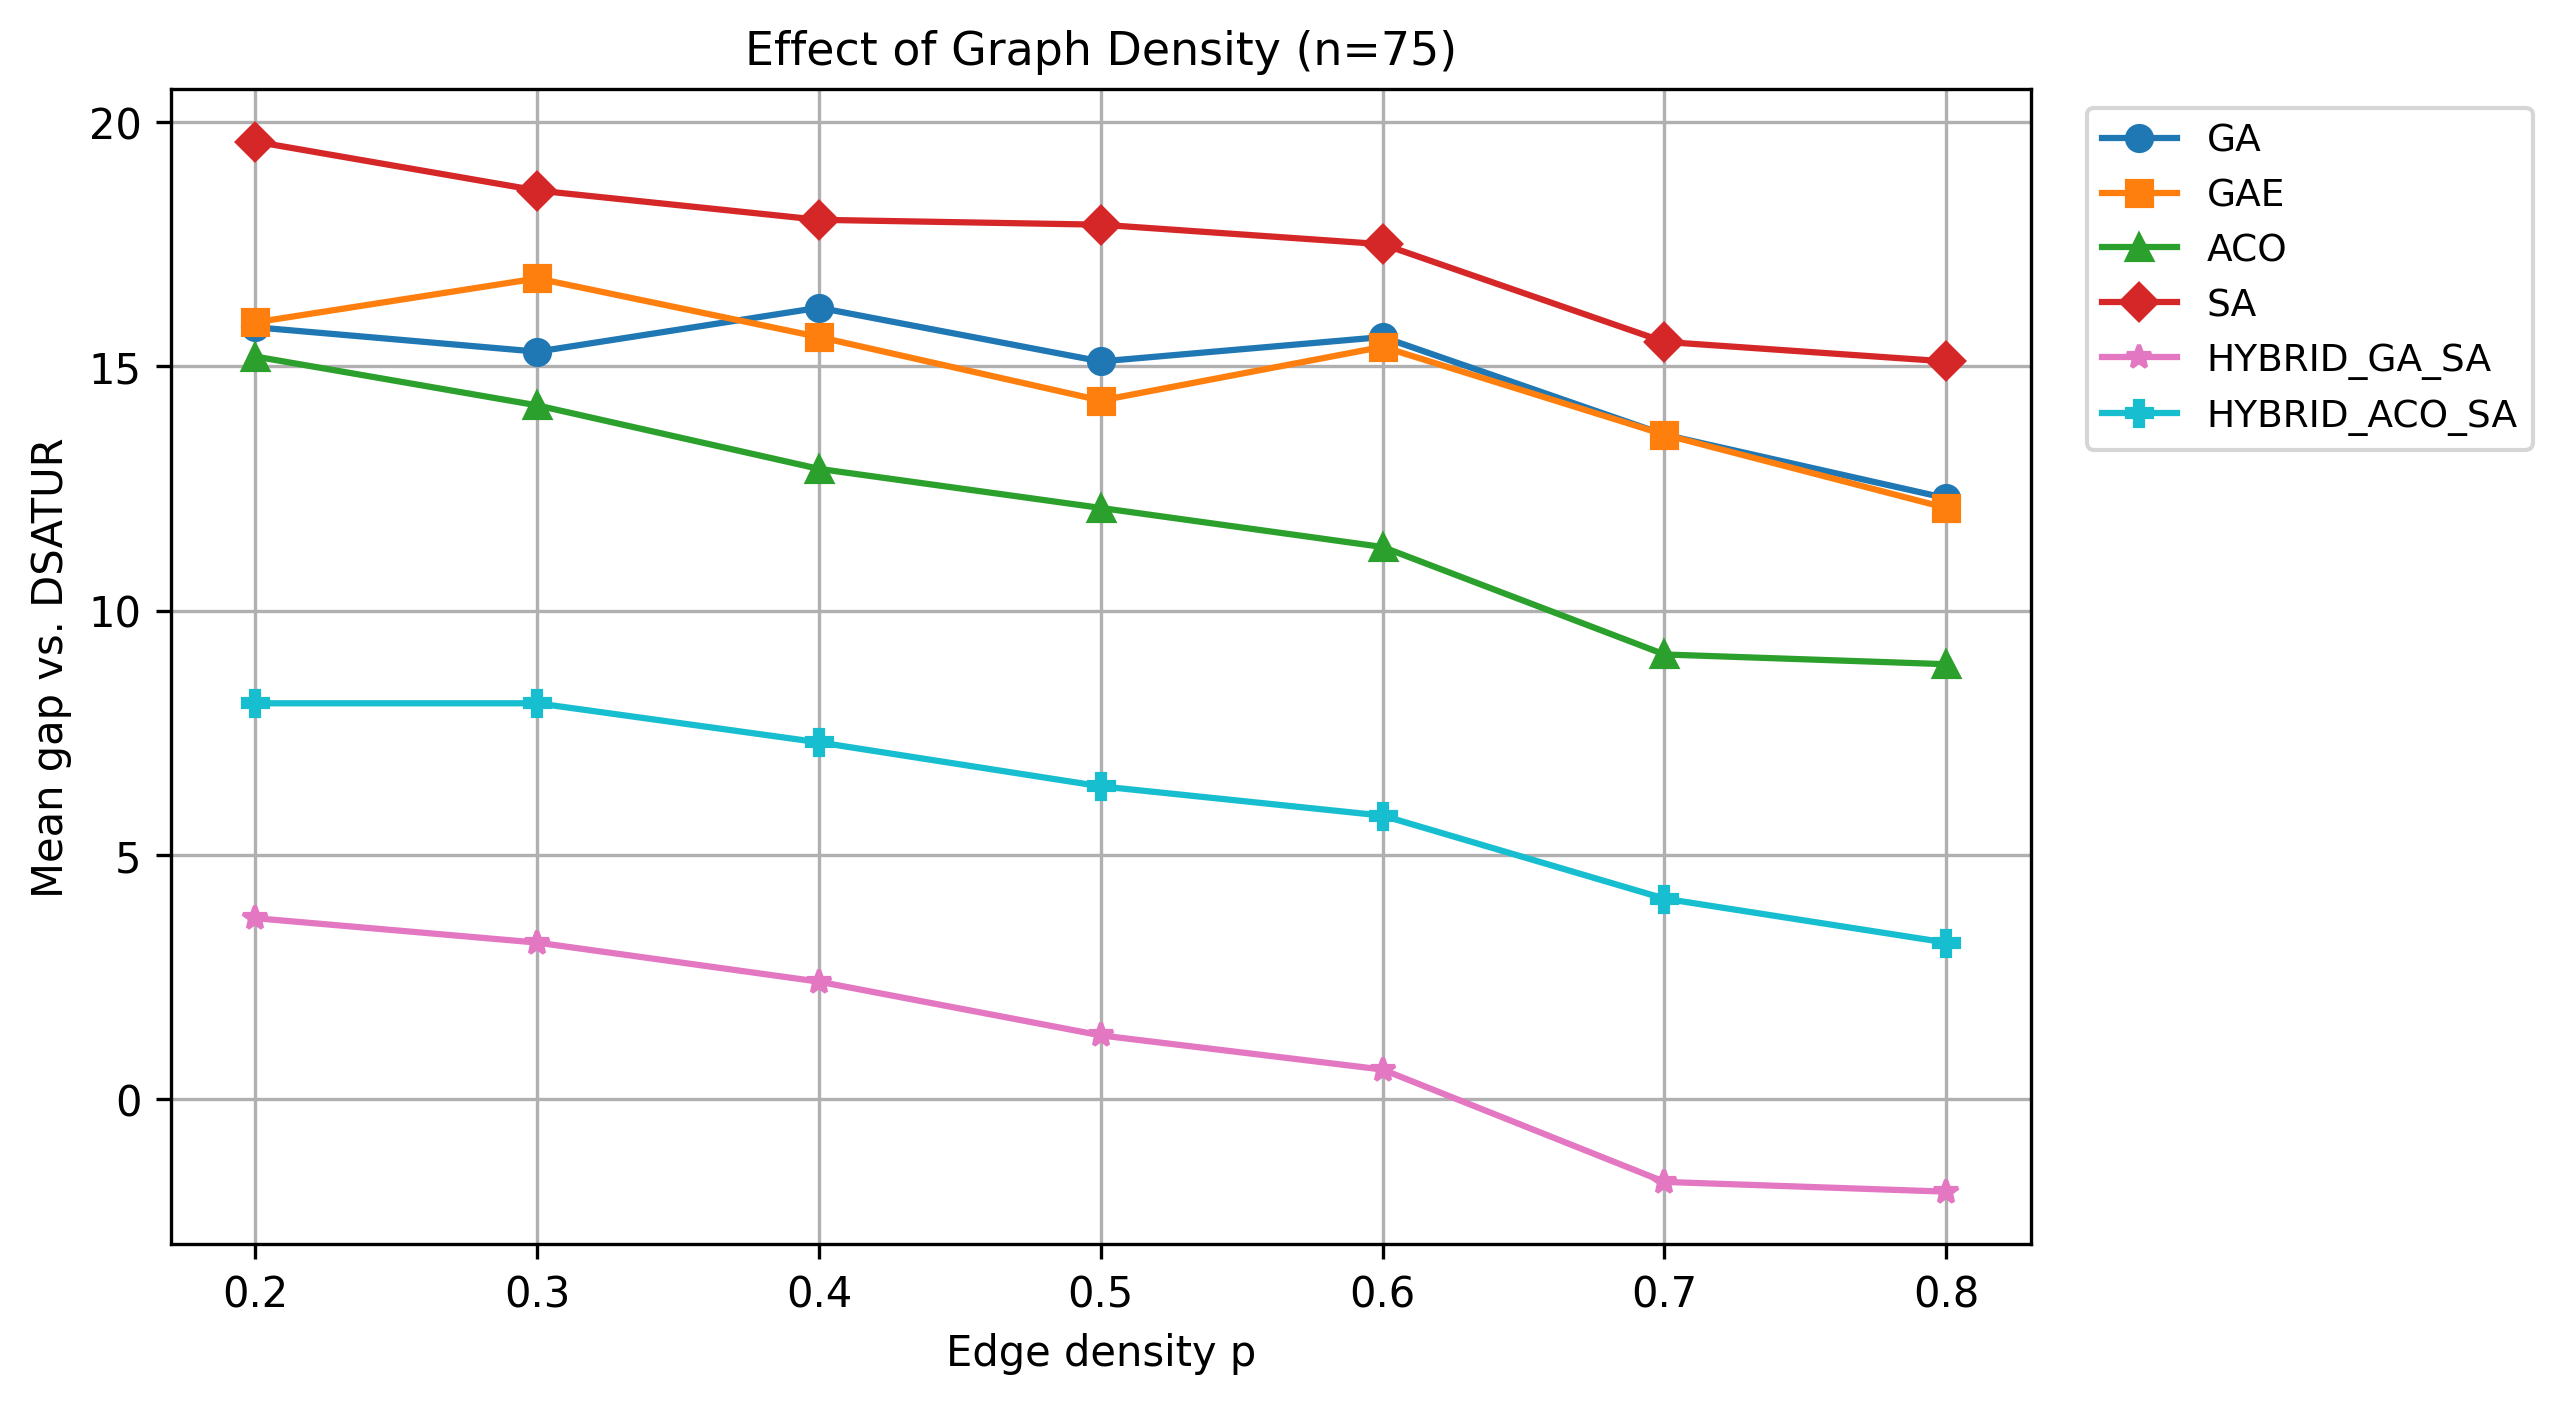
\includegraphics[width=\textwidth]{../results/figures/density_sweep.png}\\[0.3em]
{\small Mean gap vs.\ edge density $p$ ($n{=}75$)}
\end{column}
\end{columns}

\vspace{0.3em}
\footnotesize
\begin{itemize}
  \item \textcolor{algaecolor}{GAE} now has the highest variance at large $n$ (std $\approx 6.6$ at $n{=}200$), narrowly ahead of \textcolor{algacolor}{GA} ($\approx 6.0$) — both unreliable at large $n$
  \item \textcolor{algacocolor}{ACO} most consistent (lowest $\sigma$) but far from optimal; \textcolor{hybridacocolor}{Hybrid ACO+SA} nearly as tight while much closer to optimal
  \item All algorithms improve vs.\ DSATUR as density $p$ increases; \textcolor{hybridgacolor}{Hybrid GA+SA} even turns negative (beats DSATUR) for $p \geq 0.7$
\end{itemize}
\normalsize

\end{frame}

% ── Slide 14: Results — DIMACS Benchmark ─────────────────────────────────────────
\begin{frame}{Results: DIMACS Benchmark (Known $\chi(G)$)}

\begin{columns}[T]
\begin{column}{0.56\textwidth}
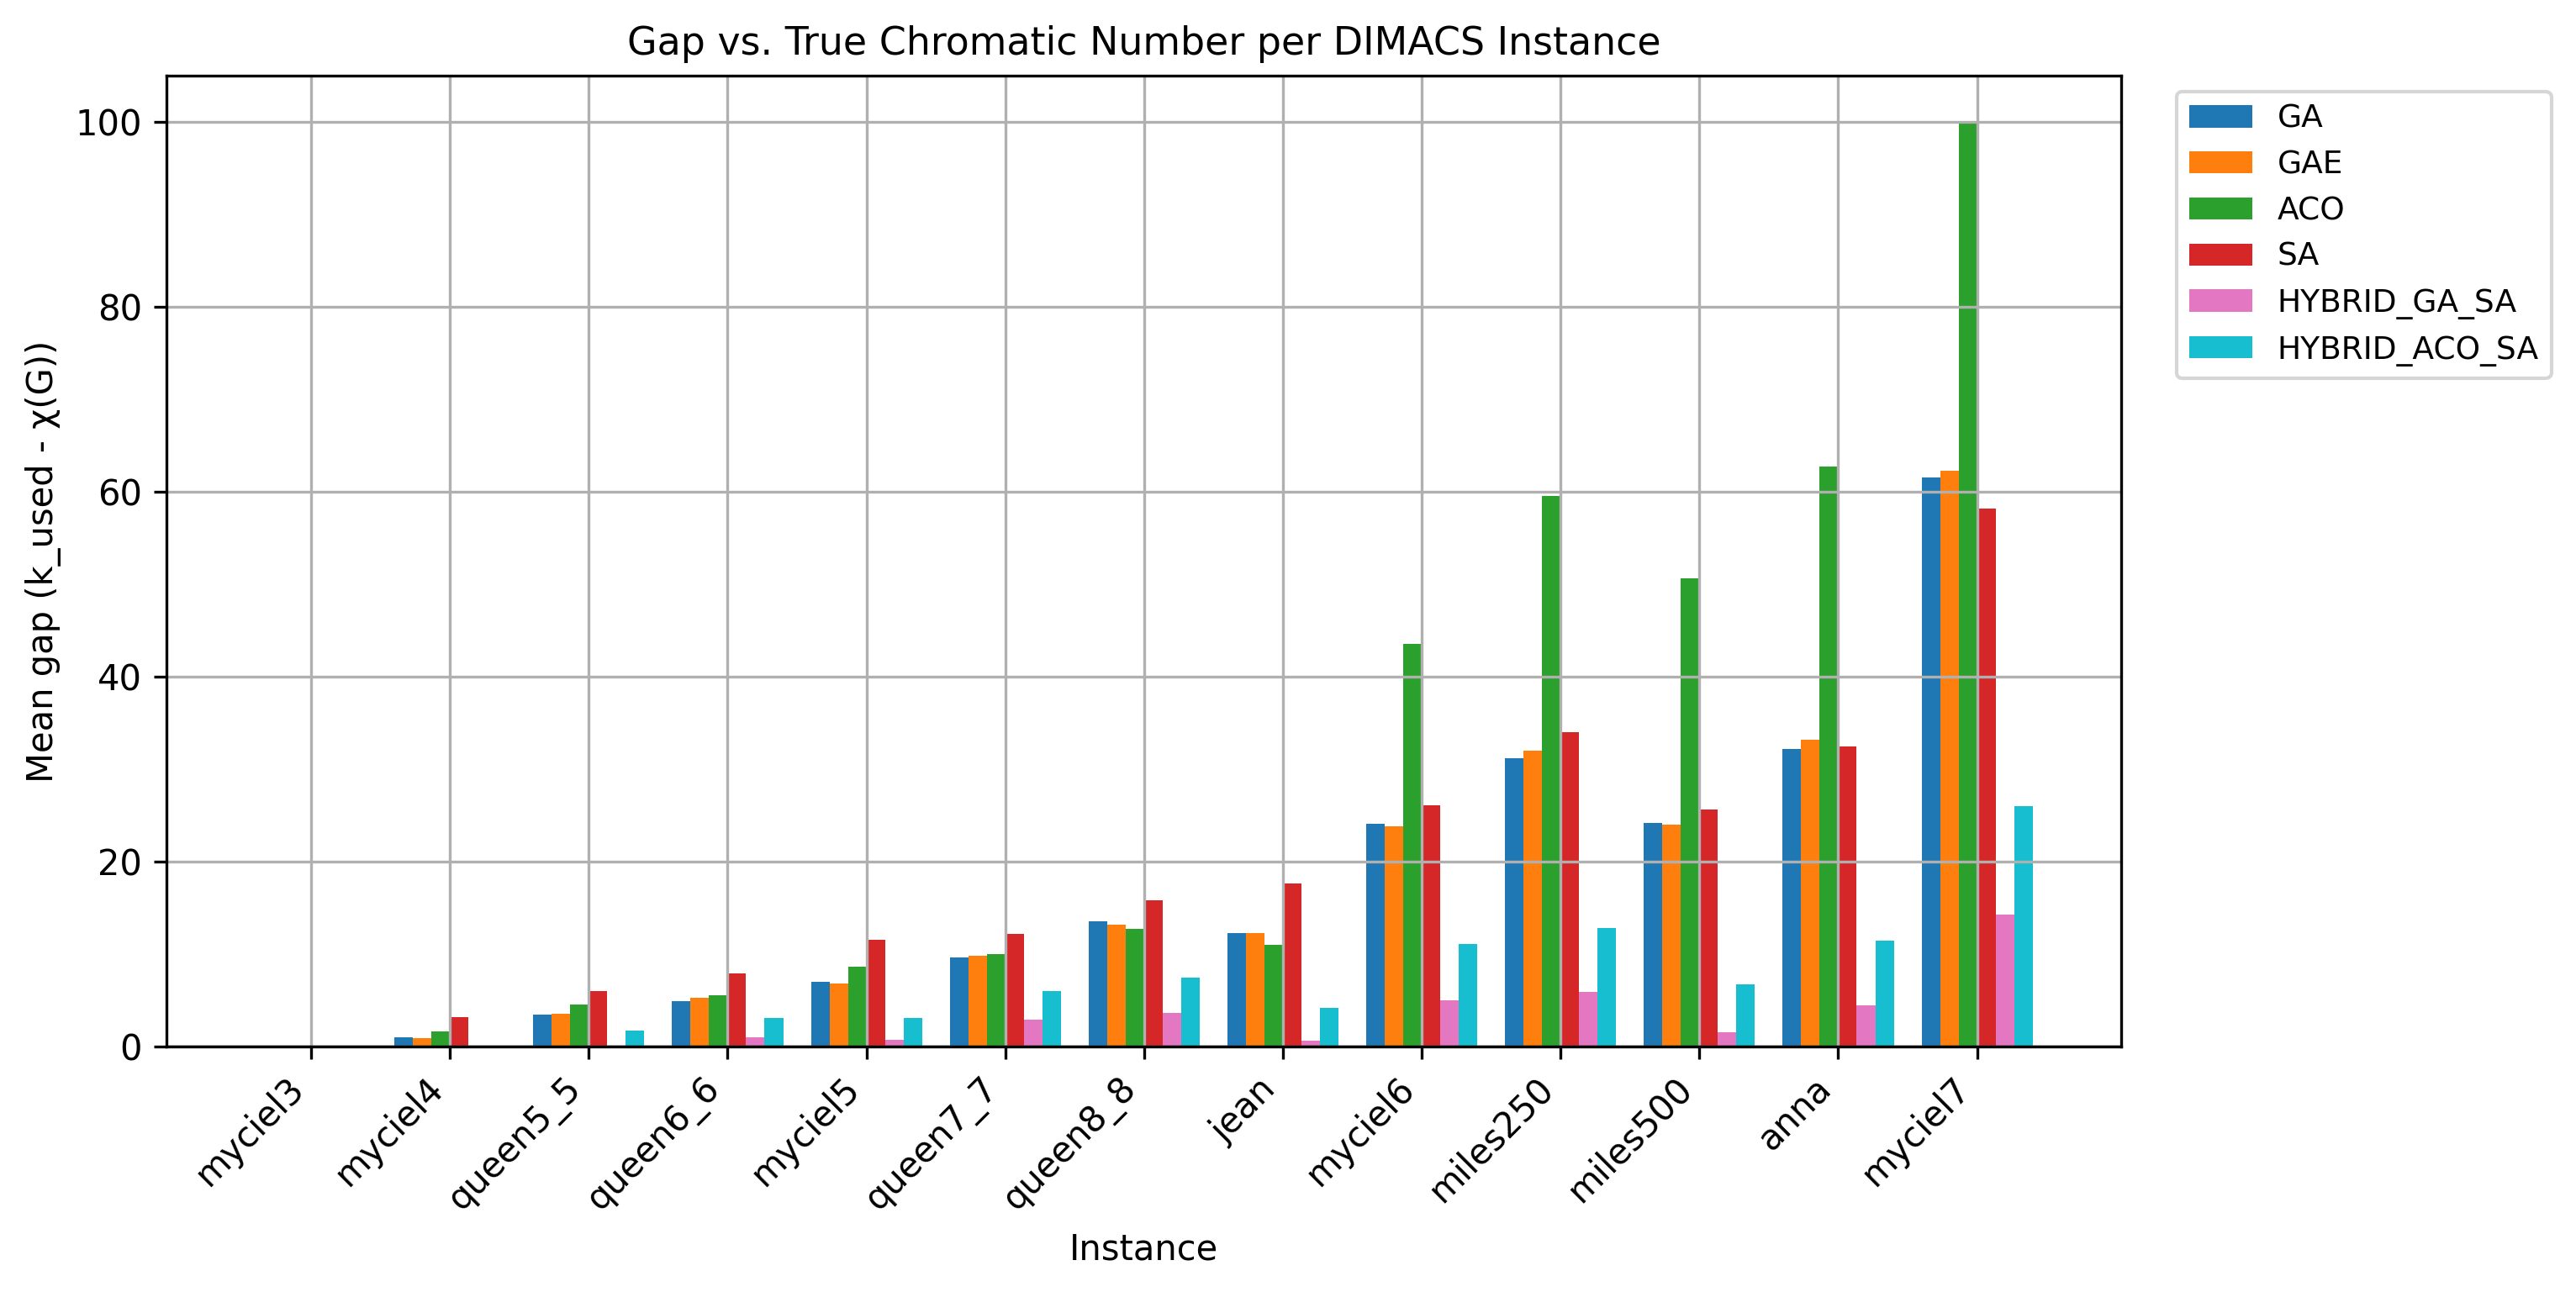
\includegraphics[width=\textwidth]{../results/figures/dimacs_gap.png}
\end{column}

\begin{column}{0.41\textwidth}
\footnotesize
\vspace{0.2em}
13 fixed instances (myciel3–7, queen5\_5–8\_8, miles250/500, anna, jean); $\gap_{\text{true}} = \kused - \chi(G)$\\[0.3em]

\begin{itemize}
  \item \textcolor{hybridgacolor}{\textbf{Hybrid GA+SA}} best on 12/13 instances; mean $\gap_{\text{true}}=3.1$ vs.\ 17.3–19.3 for GA/GAE/SA, 28.5 for plain ACO
  \item \textcolor{hybridacocolor}{Hybrid ACO+SA} mean $\gap_{\text{true}}=7.2$ — a $4\times$ improvement over plain ACO
  \item Gap widens most on the largest instance \texttt{myciel7} ($n{=}191$): ACO reaches $\gap_{\text{true}}{=}100$ vs.\ 14.3 for Hybrid GA+SA
  \item 100\% feasibility across all DIMACS runs
\end{itemize}
\normalsize
\end{column}
\end{columns}

\vspace{0.2em}
{\footnotesize Same ranking as the random-graph sweep: hybridising with SA refinement is the single biggest lever on solution quality.}

\end{frame}

% ── Slide 15: Summary ────────────────────────────────────────────────────────
\begin{frame}{Summary}

\renewcommand{\arraystretch}{1.3}
\centering
\footnotesize
\begin{tabular}{>{\bfseries}l cccccc}
\toprule
 & \algbox{algacolor}{GA} & \algbox{algaecolor}{GAE} & \algbox{algacolorsa}{SA} & \algbox{algacocolor}{ACO} & \algbox{hybridgacolor}{GA+SA} & \algbox{hybridacocolor}{ACO+SA} \\
\midrule
Mean gap (all $n$)   & 22.8 & 22.6 & 20.4 & 30.7 & \textbf{2.4} & 8.0 \\
Gap at $n=200$       & 77.5 & 77.3 & 54.6 & 100.9& \textbf{10.1}& 24.1 \\
Mean runtime (s)     & 9.1  & 9.5  & \textbf{1.6} & 208.9& 324.9        & 8.2 \\
Feasibility          & 100\%& 99.8\%& 100\%& 100\%& 100\%       & 100\% \\
Variance (large $n$) & High & Highest & Med. & \textbf{Low} & Med. & Low \\
\bottomrule
\end{tabular}
\normalsize

\vspace{1em}
\begin{columns}
\begin{column}{0.45\textwidth}
\begin{block}{Best quality}
\textcolor{hybridgacolor}{\textbf{Hybrid GA+SA}} — best mean gap and best at $n=200$, on both random graphs and DIMACS
\end{block}
\end{column}
\begin{column}{0.45\textwidth}
\begin{block}{Best quality/speed}
\textcolor{algacolorsa}{\textbf{SA}} fastest overall; \textcolor{hybridacocolor}{\textbf{Hybrid ACO+SA}} best trade-off among the refined variants
\end{block}
\end{column}
\end{columns}

\end{frame}

% ── Slide 16: Conclusions ────────────────────────────────────────────────────
\begin{frame}{Conclusions and Outlook}

\begin{columns}[T]
\begin{column}{0.50\textwidth}
\textbf{Findings}
\footnotesize
\begin{itemize}
  \item SA-based local refinement is the single biggest lever on quality: Hybrid GA+SA cuts the mean gap from 18–23 (GA/GAE/SA) to \textbf{2.4}, and the $n{=}200$ gap from $\sim$\,77 to \textbf{10.1}
  \item Elitism alone (GAE vs.\ GA) barely moves the needle by comparison
  \item Wrapping ACO's slow construction in SA refinement (Hybrid ACO+SA) roughly quadruples its quality at $\sim$\,4\% of its runtime
  \item Same ranking holds on 13 DIMACS instances with known $\chi(G)$: Hybrid GA+SA best on 12/13
  \item Feasibility 100\% for 5/6 algorithms; GAE had 1 infeasible run out of 600 (99.8\%)
\end{itemize}
\normalsize
\end{column}

\begin{column}{0.46\textwidth}
\textbf{Directions for improvement}
\footnotesize
\begin{itemize}
  \item \textbf{GA/GAE}: seed population from DSATUR to eliminate the infeasibility phase
  \item \textbf{ACO}: vectorise construction step (NumPy); current Python loop is the bottleneck
  \item \textbf{Hybrid GA+SA}: cheapen the per-generation SA pass — now the slowest of the six despite the best quality
  \item \textbf{Hybrid ACO+SA}: already a strong cost/quality trade-off; tune \texttt{sa\_restarts} further for large $n$
  \item \textbf{All}: larger budget ($n_{\text{gen}}$, $N_{\text{iter}}$) for large $n$
\end{itemize}
\normalsize
\end{column}
\end{columns}

\vspace{0.3em}
\begin{center}

\begin{tikzpicture}
  \node[fill=ethblue,text=white,rounded corners,inner sep=8pt,font=\bfseries] {
    Code, results and cluster scripts: \url{https://github.com/easchmann/optimisation-project}
  };
\end{tikzpicture}
\end{center}

\end{frame}

\end{document}
